\documentclass[twocolumn,twoside,10pt,superscriptaddress,prl]{revtex4}
%\documentclass[showpacs,twoside,10pt,superscriptaddress,prl]{revtex4}

\usepackage{graphicx}
\usepackage{epsfig}
\usepackage{epsf}
\usepackage{amssymb}
%\usepackage{epstopdf}
\usepackage{amsmath}
\usepackage{amsthm}
%\usepackage[colorlinks=true,dvipdfm]{hyperref}

\newcommand{\bra}[1]{\langle #1|}
\newcommand{\ket}[1]{|#1\rangle}

%opening


\begin{document}

\title{Schema of how to do in experiment}


\maketitle

\begin{figure}[htb]
\begin{center}
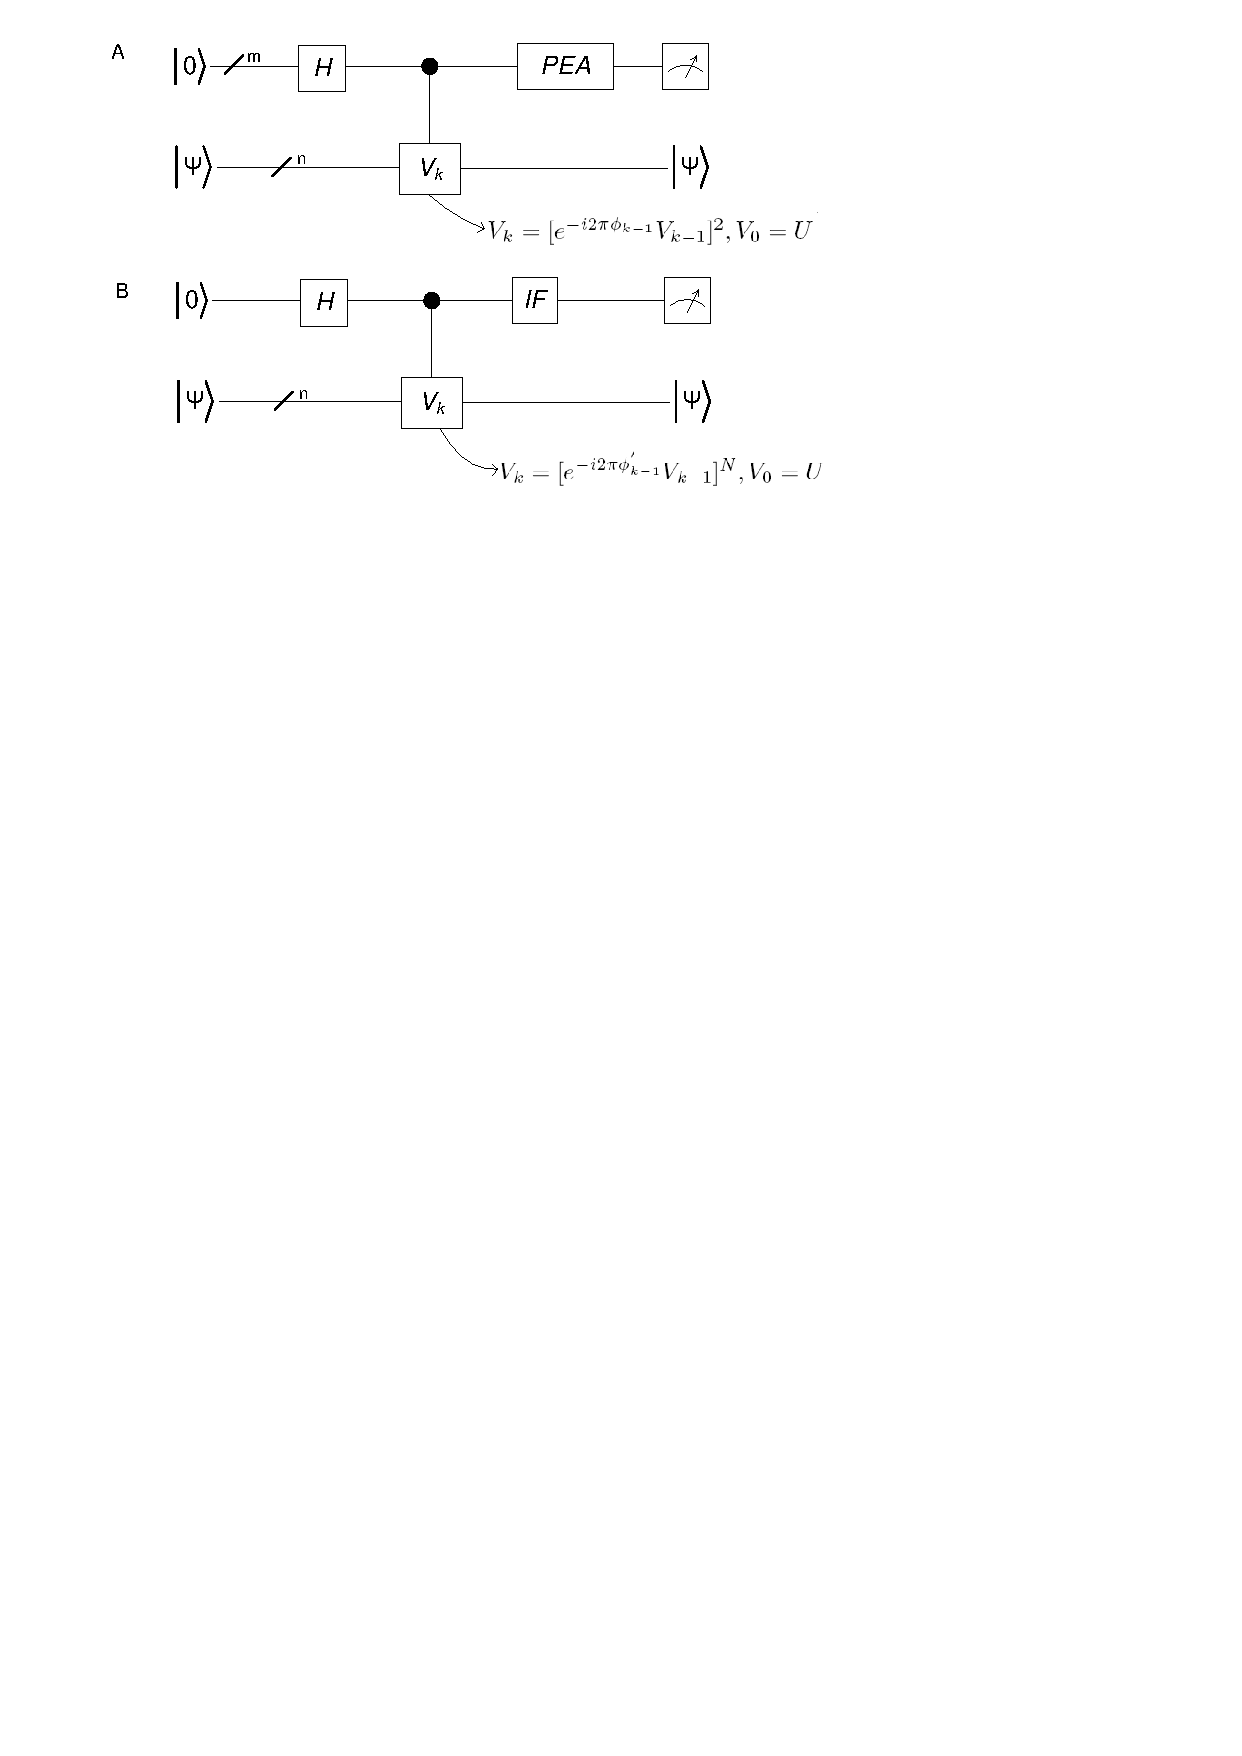
\includegraphics[width= 0.99\columnwidth]{demo_circuit}
\end{center}
\caption{Schemes to calculate the ground energy of molecules.(A) the
schematic diagram of Aspuru-Guzik's proposal. (b) the diagram of our
modified schema. PEA is phase estimate algorithm and IF is
Interferometer. both the schemes should be iterated for many times
and for each iteration the energy is calculated with a few bits of
precision} \label{Sim}\label{circuit1}
\end{figure}

the overall formula is
$$
V_k = [e^{-i2\pi\phi^{'}_{k-1}}V_{k-1}]^N,V_0=U
$$
Note that

1.$\phi$ is the overall real phase we are to measure

2.$\phi^{exp}_k$ is the value we get in the experiment in the $k$th
 iteration.

3.$\phi^{real}_k$ is the real value in the $k$th iteration that we
are to measure. so $\phi=\phi^{real}_0$

4.$\phi_{errbound}=0.014$ is the error bound which means
$|\phi^{real}_k-\phi^{exp}_k|\leq \phi_{errbound}$.

5.$\phi^{'}_k=max\{\phi^{exp}_k-\phi_{errbound},0\}$ is the value we
use to generate the operator $V_{k+1}$ in the  $k+1$-th iteration.

6.in our experiment, $N=8$.

so in the first iteration,
$$
V_0 = U;
$$

in the second iteration,
\begin{eqnarray}
V_1&=&[e^{-i2\pi\phi^{'}_0}V_0]^8\\
&=&U^8*e^{-i2\pi(\phi^{'}_0*8)}\\
\phi^{'}_0&=&max\{\phi^{exp}_0-\phi_{errbound},0\}
\end{eqnarray}

in the third iteration,
\begin{eqnarray}
V_2&=&[e^{-i2\pi\phi^{'}_1}V_1]^8\\
&=&[e^{-i2\pi\phi^{'}_1}U^8*e^{-i2\pi(\phi^{'}_0*8)}]^8\\
&=&U^{64}*e^{-i2\pi(\phi^{'}_0*64)}e^{-i2\pi(\phi^{'}_1*8)}\\
\phi^{'}_1&=&max\{\phi^{exp}_1-\phi_{errbound},0\}
\end{eqnarray}

So for all the iterations
\begin{eqnarray}
V_k&=&U^{8^k}*\prod^{k-1}_{j=0}{e^{-i2\pi(\phi^{'}_j*8^{k-j})}}\\
\phi^{'}_k&=&max\{\phi^{exp}_k-\phi_{errbound},0\}
\end{eqnarray}

CAUTION: THE iteration number $k$ starts from 0, not 1!!!!





\end{document}
